\section{\textbf{Methodology}}
The key objective of our project is to design a system that can classify suspicious and non-suspicious text. \textbf{Fig} \ref{fig:proposed_model} shows an abstract view of our suspicious text detector classifier.

\begin{figure}[h!]
\centering
  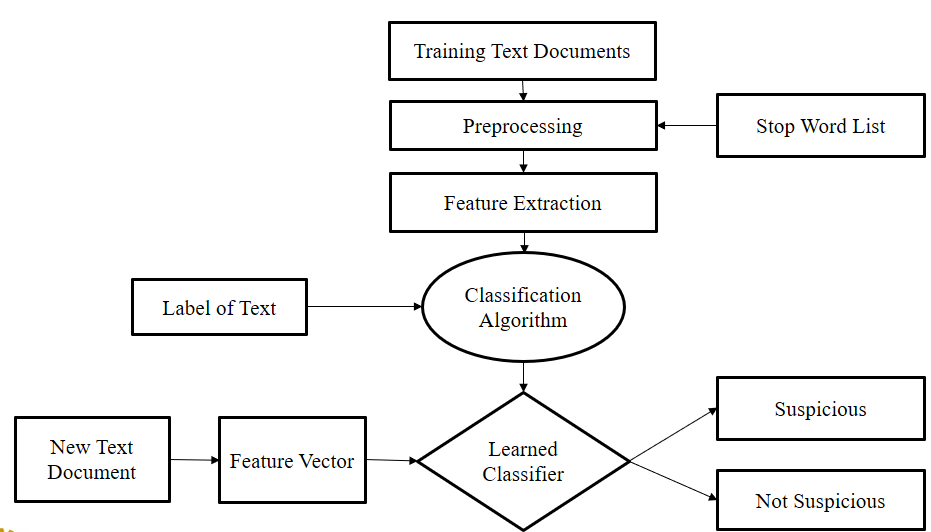
\includegraphics[scale=0.365]{Figures/proposed_model.PNG}
  \caption{ Model for Suspicious Text Detection}
  \label{fig:proposed_model}
\end{figure}

We have implemented this system by using different supervised machine learning algorithms. As a supervised classification problem, our whole system is classified into two phases one is training phase and another is testing phase.
\subsection{\textbf {Training Phase}}
In training set each document is labeled as either suspicious or non suspicious. Training phase of suspicious text detector includes five steps:
\subsubsection{\textbf{Training Set Preparation}}
Training set is divided into positive set (suspicious texts) and negative set (non suspicious texts).
\subsubsection{\textbf{Text Preprocessing}}
All texts are preprocessed by the preprocessor in order to remove inconsistencies for dataset. In our system the word which has no contribution in deciding whether a text is suspicious or not suspicious is referred as stop word. Such words are removed form the text by matching with a stop word list. 
\subsubsection{\textbf{Feature Extraction}}
A word list is created by the tokenizer by tokenizing the main body of a text. Word frequencies is used as features in this system. Bag of words model is used to represent the features. Our feature space is a two dimensional array where rows represents each text of the corpus and columns represents unique words available in the corpus. Each cell of the array represents the number of time a specific word occurs in a specific text.
\subsubsection{\textbf{Training the Suspicious Text Detector}}
It is most important part of our whole system. If we able to train our model correctly than the output will be better. Five different machine learning algorithms is used to train our model. 
\vspace{0.3cm}

\textbf{Naive Bayes}\cite{yoo2015classification} can be defined as Bayes theorem with a conditional independency assumption that all variables $A_{1},A_{2},...,A_{n}$ in a given category $C$ are conditionally independent with each other given $C$. 
According to Bayes rule for a text document $(T)$ and class $(C)$ we can write,
\begin{equation}
    P(C|T) = \frac{P(T|C)P(C)}{P(T)}
\end{equation}
The class we are looking for to assign this document is out of all classes the one that maximizes the probability of that class given the document.
\begin{equation}\label{eq:11}
 \begin{aligned}
     C_{MAP} & = argmax P(C|T) \\     & = argmax \frac{P(T|C)P(C)}{P(T)}
\end{aligned}
\end{equation}
So final equation for Naive Bayes Classifier is,
\begin{equation}
     C_{MAP} = argmax P(X_{1},X_{2},...,X_{n}|C)P(C)
\end{equation}
\vspace{0.1cm}

\textbf{SVM}\cite{wei2012text} analyze data used for classification and regression analysis. SVM can perform linear classification as well as non-linear classification using kernel trick. For linear classification cost function can be written as,
\begin{equation}
    \label{cost_function_svm}
    \frac{1}{n}\sum_{i=1}^{n}\max{(0,1-y_{i}(w.x_{i}-b))} + \lambda (\lVert \mathbf{w} \rVert)^2
\end{equation}
The parameter $\lambda $ in above equation determines the trade-off between increasing the margin-size and ensuring that the samples lie on the correct side of the margin.

For non-linear classification with SVM kernel trick is used. Some common kernel tricks used in machine learning are,
\begin{itemize}
    \item Gaussian radial basis function:
    \begin{equation}
         k(x_{i}, x_{j}) = \exp{(-\gamma(\lVert \mathbf{x_{i}-x_{j}} \rVert)^2)}
    \end{equation}
    \item Polynomial Kernel (homogeneous):
    \begin{equation}
        k(x_{i}, x_{j}) = (x_{i}\cdot x_{j})^d
    \end{equation}
     \item Polynomial Kernel (inhomogeneous):
     \begin{equation}
         k(x_{i}, x_{j}) = (x_{i}\cdot x_{j}+1)^d
     \end{equation}
\end{itemize}
\vspace{0.1cm}

A \textbf{Decision Tree}\cite{chavan2014survey} has two types of nodes one is external and another is internal. Decision classes are represented by external node of a decision tree. Internal nodes corresponds to attribute which are used for making decision by decision tree algorithm. Decision tree is simple to build and as it is a inductive algorithm it can be interpreted easily. Entropy is used to calculate the homogeneity of a sample. To build a decision tree, we need to calculate two types of entropy using as follows,
\begin{enumerate}
    \item Entropy using one attribute :
    \begin{equation}
         E(S) = \sum_{i=1}^{c}-P_i \log_2P_i
    \end{equation}
    \item Entropy using two attributes :
    \begin{equation}
        E(S) = \sum_{c\epsilon X}{}P(C)E(C) 
    \end{equation}
    
\end{enumerate}


\textbf{Logistic Regression}\cite{sharma2015active} is a binary classification model that predicts a binary outcome based on some features. The output of logistic regression depends on logistic function. The definition of logistic function or hypothesis function is,
\begin{equation}
    h_{\theta}(x) =  \frac{1}{1+\exp({-\theta^T x})}
\end{equation}
Cost function for Logistic regression is,
\begin{equation}
    J(\theta) = \frac{1}{m}\sum_{i-1}^{m}cost(h_{\theta}(x^{i}),y^{i})   
\end{equation}

\[
cost(h_{\theta}(x), y) = 
\begin{cases}
    -\log (h_{\theta}(x)) & \texttt{if } y = 1\\
     -\log (1-h_{\theta}(x)) & \texttt{if } y = 0
\end{cases}
\]
Here,\\
$m = $ Number of training examples.\\
$h_{\theta}(x^{i}) = $ Hypothesis function of $i_{th}$ training example\\
$y^i = $ Input label of $i_{th}$ training example.

\vspace{0.3cm}

\textbf{KNN}\cite{harisinghaney2014text} is a non-parametric method used for
classification and regression. K nearest neighbors is a simple algorithm that stores all available cases and classifies new cases based on a similarity measure (e.g., distance functions). Most commonly used three different distance function of K-NN are,

\begin{enumerate}
    \item Euclidean distance function :
    \begin{equation}
        \sqrt{\sum_{i=1}^{k}(x_i-y_i)^2}
    \end{equation}
    \item Manhattan distance function :
    \begin{equation}
         \sum_{i=1}^{k}\abs{(x_i-y_i)}
    \end{equation}
    \item Minkowski distance function :
    \begin{equation}
        ({\sum_{i=1}^{k}(\abs{x_i-y_i})^q)})^\frac{1}{q}
    \end{equation}
    
\end{enumerate}
All three distance measures are only valid for continuous variables.

\subsubsection{\textbf{Saving the Model}}
The result of the training phase is used in testing phase. The result is saved as a model which contains knowledge for classifying a new text document into suspicious or non suspicious category.

\subsection{\textbf{Testing Phase}}
Testing is the most important phase for any machine learning model. Classification accuracy of the text classifier is calculated in testing phase. In our system testing phase is quite similar as training phase but in this part our learned classifier model is used for predicting. Sample texts are taken to test the system. After processing, using feature extraction methods features are extracted from the texts. Our classifier model use this features to classify a text as suspicious and non suspicious.